\xchapter{Publicização de software acadêmico de análise estática}{} 
\label{estudo1}

Este capítulo apresenta um estudo sobre a publicização de software acadêmico
de análise estática divulgado nas conferências ASE - Automated Software Engineering, e 
SCAM - Working Conference on Source Code Analysis \& Manipulation, até o ano de 2015.
Nossa revisão de literatura identificou
60 projetos de software de análise estática
publicados em artigos nessas duas conferências, e caracterizou estes
projetos em relação a sua publicização, em termos de disponibilidade para
download, acesso ao código fonte, forma de distribuição e licença.

A seção \ref{estudo1:introducao} apresenta a motivação para realização do estudo,
a seção \ref{estudo1:escopo} define o escopo, descreve o objetivo e apresenta as questões de pesquisa,
a seção \ref{estudo1:planejamento} apresenta um planejamento do estudo,
as seções \ref{estudo1:preparacao} e \ref{estudo1:coleta} apresentam detalhes sobre a preparação e execução da coleta de dados,
as seções \ref{estudo1:analise} e \ref{estudo1:interpretacao} apresentam a análise e interpretação dos dados e
a seção \ref{estudo1:conclusoes} apresenta as conclusões finais deste estudo.

\section{Motivação} \label{estudo1:introducao} % {{{
%Sets the scope of the work and encourages readers to read the rest of the chapter

Software acadêmico é um termo usado para denotar
projetos de software desenvolvidos durante pesquisas científicas,
publicados na literatura acadêmica, normalmente utilizados para coleta ou
análise de dados, possivelmente com objetivo de ser utilizado por outros
pesquisadores e, em algumas ocasiões, sendo o próprio software uma contribuição
primária para a Ciência \cite{howison2011scientific}.
%
Neste contexto, a \textit{publicização} do software acadêmico, isto é,
a ação de tornar o software disponível 
a partir da URL indicada no artigo científico publicado pelos seus autores,
é fundamental.
Características importantes do software acadêmico após a sua publicização
incluem a forma em que os projetos são disponibilizados (binário ou código fonte),
os tipos de licença utilizados, e outras questões relacionadas à sua distribuição.

Há diversos projetos de software acadêmico com características e
funcionalidades parecidas, com poucos usuários, com ciclos de vida curtos, e
encerrados quando o financiamento inicial termina, bem como, comunidades
desconectadas e paralelas, incompatibilidades entre projetos de um mesmo
domínio, e tentativas aparentemente não coordenadas de ``reiniciar'' tudo ({\it re-boots}).
Em tais condições, diz-se que o software acadêmico sofre de 
{\it ``dysfunctional chaotic churn''} \cite{howison2015understanding}.

Parte deste problema tem sido atribuido a falta de treinamento em boas práticas
para o desenvolvimento de software de qualidade por parte dos cientistas e pesquisadores
\cite{wilson2017good}, 
e na publicização adequada do software acadêmico \cite{allen2017engineering}.
A princípio, a falta de treinamento não deveria afetar os cientistas da
Engenharia de Software, visto que estes possuem formação e acesso a práticas de
desenvolvimento e estão inseridos num contexto voltado para a compreensão e
melhoria dos processos de desenvolvimento de software, tanto do ponto de vista
teórico, quanto prático.

Sabendo disso, e atentando para o fato de que grande parte do desenvolvimento
de software acadêmico é realizado pelos próprios cientistas
\cite{hettrick2014uk, momcheva2015software}, surge a preocupação de avaliar 
a publicização do software acadêmico desenvolvido nas pesquisas de Engenharia de
Software e se apresenta sintomas de ``dysfunctional chaotic churn'' conforme
percebido por \citeonline{howison2015understanding}.

% }}}

\section{Escopo} \label{estudo1:escopo} % {{{

Projetos de software acadêmico de análise estática publicados nas 
conferências ASE e SCAM 
são nosso principal objeto de estudo.
Queremos saber quantos projetos de software acadêmico de análise estática publicados
nas conferências ASE e SCAM foram publicizados adequadamente, se permanecem disponíveis e 
quais são as informações que podem ser obtidas.

O objetivo da pesquisa está definido segundo a estrutura GQM \cite{basili1994goal}.

\subsection{Definição do Objetivo}

\begin{description}
  \item{\bf Objeto de estudo.}
     O objeto de estudo são projetos de software acadêmico de análise estática
     publicados em artigos científicos e sua publicização em termos de
     disponibilidade, licença e distribuiçao, conforme definido na
     seção~\ref{estudo1:introducao}.
  \item{\bf Propósito.}
    O propósito do estudo é caracterizar a publicização de cada software
    acadêmico de análise estática publicado nas conferências selecionadas.
    O estudo contribuirá para a análise da desordem disfuncional caótica no
    domínio de análise estática.
  \item{\bf Perspectiva.}
    A perspectiva considerada é a do cientista usuário final, isto é, o
    pesquisador que deseja saber se há DDC no software acadêmico do domínio de
    interesse. A perspectiva a ser considerada é a do pesquisador que deseja
    conhecer ferramentas de análise estática para uso em sua pesquisa.
  \item{\bf Foco de qualidade.}
    O principal foco de qualidade estudado é a publicização do software
    acadêmico de análise estática, com ênfase nos aspectos de disponibilidade
    de URL com infornações sobre o projeto, especialmente sobre acesso ao
    código fonte.
  \item{\bf Contexto.}
    O estudo foi conduzido com artigos que apresentam software acadêmico de
    análise estática, publicados das conferências de Engenharia de Software ASE
    e SCAM.
\end{description}

\subsection{Sumário da Definição}

Analisar os \textit{projetos de software acadêmico de análise estática} publicados
com o propósito de \textit{caracterizá-los} 
com respeito a sua \textit{publicização}
na perspectiva de \textit{cientistas usuários finais}
no contexto das \textit{conferências de Engenharia de Software ASE e SCAM}.

\subsection{Questões de Pesquisa}

Neste estudo as seguintes questões de pesquisa, a respeito dos projetos de
software acadêmico de análise estática publicados nas conferências ASE e SCAM,
e sua publicização serão investigadas:

\newcommand{\EstudoUmQuestaoUm}{
  Os projetos de software acadêmico de análise estática publicados nas
  conferências ASE e SCAM possuem alguma presença oficial online?
}
\newcommand{\EstudoUmQuestaoDois}{
  Os projetos de software academico de análise estática publicados nas
  conferências ASE e SCAM estão disponíveis para download?
}
\newcommand{\EstudoUmQuestaoTres}{
  É possível ter acesso ao código fonte dos projetos de software de análise
  estática publicados nas conferências ASE e SCAM?
}
\newcommand{\EstudoUmQuestaoQuatro}{
  Os projetos de software com código fonte disponível usam licenças de software
  livre ou código aberto?
}

\begin{description}
  \item [Q1:] \EstudoUmQuestaoUm

    Por presença oficial online entende-se site ou repositório oficial do
    projeto, um endereço URL com informações do software, geralmente mantido
    pelos próprios autores do software.

  \item [Q2:] \EstudoUmQuestaoDois

    Com esta questão queremos saber se é possível obter uma cópia online do
    software de forma que autores independentes possam utilizar e avaliar
    o software, seja com fins de reprodutibilidade de estudos utilizando o
    software, seja para fins de novas pesquisas com o apoio do software.

  \item [Q3:] \EstudoUmQuestaoTres

    Com esta questão queremos saber se pesquisadores e interessados no conhecimento
    empregado na construção do software e presente no próprio código fonte terá acesso
    a este conhecimento, que usualmente faz parte da própria pesquisa, o acesso
    ao código fonte é útil também para aqueles que tenham interesse no uso, eventuais
    adaptações ou correções pode ser necessário para executar em outros ambientes
    ou sistemas operacionais.

  \item [Q4:] \EstudoUmQuestaoQuatro

    Com esta questão queremos saber se os projetos possuem permissão explícita
    para contribuição via código fonte de forma que possam ser adaptados para
    atender necessidades emergentes e que estas adaptações possam também ser
    distribuídas livremente.
\end{description}

\subsection{Métricas}

Para responder às questões de pesquisas, as seguintes métricas serão usadas:

\begin{enumerate}
  \item Número de projetos com identificação de nome e URL
  \item Número de projetos com URL disponível
  \item Número de projetos disponíveis para download
  \item Número de projetos com código fonte disponível
  \item Número de projetos usando licenças de software livre ou código aberto
\end{enumerate}

% }}}

\section{Planejamento do Estudo} \label{estudo1:planejamento} % {{{

Este estudo foi realizado em duas etapas principais, conforme ilustrado na
Figura \ref{estudo1-etapas}. Na primeira etapa, uma revisão da literatura
foi realizada, com o objetivo selecionar
artigos com publicação de software acadêmico de análise estática. 
Na segunda etapa, os projetos de software selecionados foram caracterizados
em relação à sua publicização.

\begin{figure}[h]
  \center
  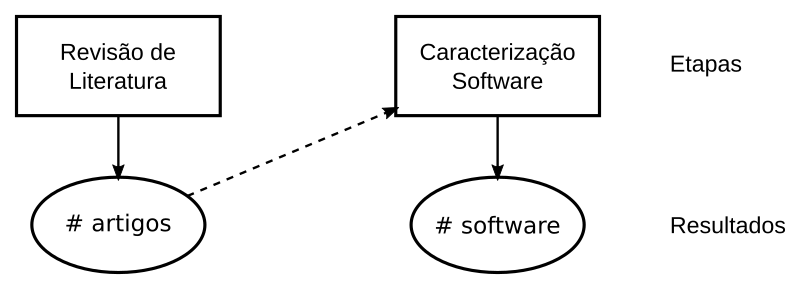
\includegraphics[scale=0.4]{imagens/estudo1-etapas.png}
  \caption{Etapas do estudo e seus resultados}
  \label{estudo1-etapas}
\end{figure}

\subsection{Revisão de literatura com publicação de software de análise estática}

O objetivo da revisão de literatura realizada foi encontrar artigos mencionando
software de análise estática entre os resultados do estudo. A revisão foi
organizada em três passos, detalhados a seguir.

\begin{description}

  \item [Passo 1: Escopo]

Este passo teve como objetivo a seleção das conferências a serem utilizadas como fonte dos
artigos para a revisão de literatura. 
Para cada conferência, todas as publicações serão selecionadas e
incluídas no conjunto inicial de artigos da revisão, iniciando pela primeira
edição de cada conferência indo até a última edição disponível no ano da execução da revisão.

As conferências devem ser selecionadas tendo em vista aumentar e potencializar
o número total de projetos de software acadêmico do domínio de aplicação de
interesse do estudo, neste caso, análise estática. Deve-se buscar
preferencialmente conferências com bom histórico de publicações sobre o domínio
de aplicação do estudo.

É importante investigar o histórico de cada conferência com atenção ao nome do
evento em cada edição; não é raro que conferências com muitos anos de
existência mudem de nome ao longo do tempo. Nestes casos, deve-se adotar o nome
da conferência mais recente e considerar todas as edições anteriores com este
mesmo nome.

Uma vez definidos a data limite e as conferências, deve-se fazer o download de
todos os artigos até a data limite, e os arquivos devem ser organizados em pastas
por nome e ano da conferência. Os títulos de todos os artigo, a correspondente
conferência e o ano de publicação devem ser registrados e armazenados em
arquivos ou banco de dados. Neste estudo fizemos uso do
LibreOffice Calc\footnote{\url{https://www.libreoffice.org}}.

  \item [Passo 2: Triagem Automática]

O escopo definido no passo anterior irá, potencialmente, resultar num enorme
conjunto de artigos para revisão. Assim, o objetivo da triagem automática é reduzir o tamanho deste
conjunto, mantendo apenas as publicações relevantes para os objetivos do estudo.

A triagem é realizada por meio de uma busca textual no conteúdo de cada artigo. A
busca deve ser realizada de forma automática com auxilio de ferramentas de
software para busca textual em conteúdo de arquivos pdf, com base em um
conjunto de palavras-chave representando os critérios de inclusão da triagem.
Apenas os artigos combinando com todos os critérios serão incluídos, conforme
Tabela \ref{criterios-triagem}.

\begin{table}[h]
\caption{Critérios de inclusão e palavras-chave para a triagem de artigos.}
\centering
\begin{tabular}{ l l }
  \hline
  Critério                                 & Palavras chave                        \\
  \hline
  Menciona projeto, software ou ferramenta & {\tt tool} ou {\tt framework}         \\
  Disponibiliza download do projeto        & {\tt download} ou {\tt available}     \\
  Identifica URL do projeto                & {\tt http} ou {\tt ftp}               \\
  Domínio de análise estática              & {\tt static analysis} ou {\tt parser} \\
  \hline
\end{tabular}
\label{criterios-triagem}
\end{table}

Se um determinado artigo não atender a algum dos critérios, ele será
excluído. Ao final da triagem, espera-se obter um conjunto reduzido
de artigos, contendo apenas as publicações relevantes para o objetivo
deste estudo.

  \item [Passo 3: Extração]

Os artigos incluídos serão inspecionados manualmente em busca de software acadêmico de
análise estática entre os resultados do estudo. Os critérios de inclusão desta etapa têm
como objetivo incluir apenas os projetos de software identificados minimamente
pelos seus autores com nome e URL para download, conforme Tabela
\ref{criterios-extracao}.

\begin{table}[h]
\caption{Critérios de inclusão para o passo de extração dos artigos (adaptado de \citeonline{howison2016software}).}
\centering
\begin{tabular}{ l p{12cm} }
  \hline
  Critério         & Explicação \\
  \hline
  Identificável    & É possível identificar um projeto de software entre as contribuições do artigo? (ex: ``um programa que nós escrevemos``, ``nossa implementação``, ``nosso protótipo'') \\
  Disponível       & Podemos encontrar menção a URL do projeto de software para download? \\
  \hline
\end{tabular}
\label{criterios-extracao}
\end{table}

O nome e o endereço URL de cada projeto encontrado durante a inspeção manual
devem ser extraídos e armazenados junto aos dados já coletados nos passos
anteriores da revisão. A inspeção deve incluir a leitura do título, introdução,
resultados e conclusões de cada artigo e, caso necessário, outras
seções do artigo. Alguns artigos podem descrever a contribuição de software acadêmico
em seções específicas, por exemplo, em
notas de rodapé com a URL do software.

Os artigos devem ser inspecionados num ciclo, um por vez, até chegar ao útlimo
artigo dentre os selecionados no passo anterior. Ao final da extração, teremos
dados de um conjunto de projetos de software acadêmico de análise estática,
incluindo nome do projeto e URL para download. Estes dados extraídos devem ser
atualizados nos arquivos ou banco de dados já utilizados nos passos anteriores.

\end{description}

\subsection{Caracterização de software acadêmico de análise estática}

Os dados coletados na revisão de literatura, devidamente armazenados em
arquivos ou banco de dados, incluem projetos de software acadêmico de análise
estática, identificados com nome e URL, nome e ano da conferência e
título do artigo onde foi publicado.

Estes dados irão compor uma nova estrutura de armazenamento
projetada para receber informações adicionais sobre os projetos, 
extraídas de outras fontes, conforme Tabela
\ref{esquema-caracteristicas}. Essas informações serão coletadas em documentos
relacionados aos projetos, como website, manuais, repositórios e código fonte.

\begin{table}[h]
\caption{Esquema para caracterização dos projetos de software acadêmico}
\centering
\begin{tabular}{ l p{11cm} }
  \hline
  Característica           & Explicação \\
  \hline
  Nome do software         & O nome do projeto de software \\
  URL                      & Endereço web do software ou projeto, site ou repositório de código fonte, com o software disponível \\
  Título do artigo         & Título do artigo onde o software é citado como contribuição, seja principal ou secundária \\
  Nome do evento           & Nome da conferência onde o software foi publicado \\
  Ano do evento            & Ano da edição da conferência onde o artigo foi publicado \\
  Descrição do software    & A descrição do projeto de software \\
  Acesso                   & Podemos acessar a URL do projeto agora? Pode receber os seguintes valores: Sem Acesso, Acesso Pago, Acesso Gratuito \\
  Distribuição             & Como o software é distribuído e pode ser acessado? Pode receber os seguintes valores: gratis, livre, proprietário \\
  Código fonte disponível  & É possível acessar o código fonte de alguma forma? \\
  Licença                  & O software deixa explícito qual licença é distribuído? \\
  Código fonte             & Em qual linguagem de programação o software acadêmico foi desenvolvido \\
  \hline
\end{tabular}
\label{esquema-caracteristicas}
\end{table}

O primeiro documento consultado deve ser o website indicado pela URL. Esta
consulta resultará em novos documentos, como, manuais de uso, informações sobre
desenvolvimento, código fonte, notas de lançamento, entre outros. 
Tais documentos devem ser inspecionados em busca de informações para
caracterização dos projetos segundo a Tabela \ref{esquema-caracteristicas}.

A identificação da linguagem de programação em que projeto está escrito deve ser
realizada de maneira automática com apoio de alguma ferramenta de análise de
código fonte, como por exemplo, o software livre
\texttt{sloccount}\footnote{http://www.dwheeler.com/sloccount}.

% }}}

\section{Preparação} \label{estudo1:preparacao} % {{{

Nesta seção apresentamos a preparação do estudo para a revisão da literatura
e realização da coleta de
dados.

\subsection{Revisão de literatura com publicação de software de análise estática}

%\vspace*{0.25cm}
%\noindent \textbf{Revisão de literatura com publicação de software de análise estática}

\begin{description}
  \item [Passo 1: Escopo]

Seguindo o planejamento descrito em \ref{estudo1:planejamento}, definimos como
fonte de busca as conferências SCAM\footnote{\url{http://www.ieee-scam.org}}
({\it Source Code Analysis and Manipulation Working Conference}) e
ASE\footnote{\url{http://ase-conferences.org}} ({\it Automated Software
Engineering}), ambas conferências com um grande histórico de edições. Definimos
como data limite o ano de 2015.

A escolha destas duas conferências baseou-se no princípio de serem conferências
tradicionais e importantes para a área de Engenharia de Software, tendo tradição
em estudos sobre análise de software, e dessa forma, potencializando aumentar
o número de projetos de software acadêmico de análise estática encontrados
entre suas publicações.

Os artigos das duas conferências estão disponíveis para download:
as publicações da conferência SCAM estão todas disponibilizadas no IEEE, e
a conferência ASE possui algumas edições no IEEE outras na ACM. Os endereços URL
de cada edição de cada conferência estão documentadas no
repositório\footnote{\url{https://github.com/joenio/dissertacao-ufba-2016}}
dessa dissertação, apresentado em detalhes no Apêndice
\ref{reproducibilidade-do-estudo}.

Até o ano de 1996, a conferencia ASE chamava-se KBSE - Knowledge-Based Software
Engineering Conference. Teve sua primeira edição no ano de 1991 e, a partir de 1997 
passou a se chamar  ASE - Automated Software Engineering Conference.
A conferência SCAM, teve sua primeira edição no ano de 2001.

  \item [Passo 2: Triagem Automática]

Para a execução da triagem automática a partir dos
critérios definidos no planejamento (Seção \ref{estudo1:planejamento}),
implementamos um script, que utiliza como base o software livre
\texttt{pdftotext}\footnote{\url{https://en.wikipedia.org/wiki/Pdftotext}}, para
converter o conteúdo pdf dos arquivos em texto antes de realizar o filtro pelas
palavras-chave.

  \item [Passo 3: Extração]

Para a execução da extração, criamos uma planilha LibreOffice Calc para coletar os dados de cada passo da
revisão de literatura com as seguintes colunas:

\begin{description}
  \item[Evento] Nome e ano da conferência de Engenharia de Software.
  \item[Escopo] Título do artigo incluído no Passo 1: Escopo.
  \item[Triagem] 'SIM' se o artigo foi incluído no Passo 2: Triagem Automática.
  \item[Extração] 'SIM' se o artigo foi incluído na Passo 3: Extração.
  \item[Software] Nome do software identificado no artigo.
  \item[Anotações] Observações sobre o contexto em que o software é mencionado.
\end{description}

\end{description}

\subsection{Caracterização de software acadêmico de análise estática}

%\vspace*{0.25cm}
%\noindent \textbf{Caracterização de software acadêmico de análise estática.}

Nesta fase de preparação para a caracterização dos projetos, definimos a
estrutura de diretórios e nomes e formatos de arquivos utilizados para
armazenar os dados coletados. Optamos por criar arquivos no formato YAML com o
nome \texttt{software.yml} para receber os dados do projeto e outro arquivo no
formato BibTeX chamado \texttt{paper.bib} para armazenar os dados do artigo
onde o software foi publicado.

Instalamos o software livre
\texttt{sloccount}\footnote{http://www.dwheeler.com/sloccount} para coletar a
linguagem de programação em que o projeto está escrito.

% }}}

\section{Coleta de Dados} \label{estudo1:coleta} % {{{

Seguindo o planejamento e preparação descritos nas seções
\ref{estudo1:planejamento} e \ref{estudo1:preparacao}, iniciamos a coleta dos
dados, organizada em duas grandes etapas: uma de revisão de literatura, e outra
de caracterização dos projetos de software acadêmico.

\subsection{Revisão de literatura com publicação de software de análise estática}

A revisão de literatura encontrou 61 artigos com publicação de projeto de
software acadêmico de análise estática entre os 1873 artigos publicados nas
conferências ASE e SCAM. As atividades e resultados de cada passo da revisão
são representadas na Figura \ref{revisao-literatura}.

\begin{figure}[h]
  \center
  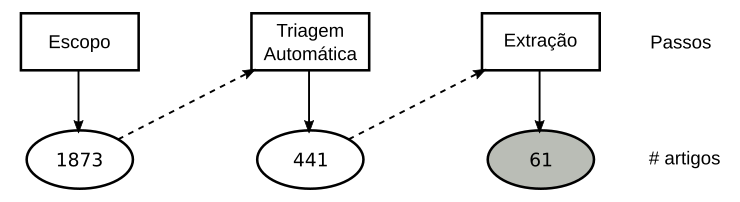
\includegraphics[scale=0.4]{imagens/revisao-literatura.png}
  \caption{Passos da revisão de literatura realizada nas conferências ASE e SCAM.}
  \label{revisao-literatura}
\end{figure}
% figura feita com base no artigo Nicolli Alves 2016, Fig 2

\begin{description}

  \item [Passo 1: Escopo]

A busca realizada nas conferências ASE e SCAM até o ano de 2015 resultou em
1873 artigos; deste total, 346 artigos são do SCAM e 1527 artigos do ASE.

  \item [Passo 2: Triagem Automática]

O filtro executado automaticamente usando os critérios definidos na fase de
preparação reduziu o conjunto de 1873 para 441 artigos, sendo 155 artigos do SCAM e
286 artigos do ASE selecionados para posterior inspeção manual.

  \item [Passo 3: Extração]

Os 441 artigos selecionados pela triagem automática foram inspecionados manualmente, tendo como guia
os critérios descritos na Tabela \ref{criterios-extracao} na fase de
planejamento. Ao final da inspeção manual, selecionamos, 61 artigos com publicação de
software acadêmico de análise estática.

\end{description}

\subsection{Caracterização de software acadêmico de análise estática}

Conforme planejado, coletamos informações adicionais 
para cada projeto de software, descritas na Tabela
\ref{esquema-caracteristicas}, consultando
documentos de cada projeto. As informações coletadas são apresentadas, de forma
resumida, na Tabela \ref{software-table}.

\begin{longtable}{l l l l l}
\caption{Software acadêmico para análise estática.}
\label{software-table} \\
  \hhline{l l l l l |}
  \hline
  \endfirsthead
  \hhline{l l l l l |}
  \hline
  \textbf{ID} & \textbf{Nome do software} & \textbf{Acesso} & \textbf{Código fonte} & \textbf{Distribuição} \\
  \hline
  \hhline{l l l l l |}
  \endhead
  \hhline{-----}
  \multicolumn{5}{c}{continua na próxima página} \\
  \hhline{-----} \endfoot
  \endlastfoot
  \textbf{ID} & \textbf{Nome do software} & \textbf{Acesso} & \textbf{Código fonte} & \textbf{Distribuição} \\
  \hline
    s1 &
      2LS &
      Gratuito &
      C++ &
      Livre \\
    s2 &
      AccessAnalysis &
      Gratuito &
      Java &
      Livre \\
    s3 &
      APIExample &
      Sem Acesso &
      - &
      - \\
    s4 &
      BEG &
      Sem Acesso &
      - &
      - \\
    s5 &
      ccJava &
      Sem Acesso &
      - &
      - \\
    s6 &
      CIVL &
      Gratuito &
      C &
      Livre \\
    s7 &
      CodeBoost &
      Gratuito &
      C &
      Livre \\
    s8 &
      CSL &
      Gratuito &
      C &
      Grátis \\
    s9 &
      CPA+ &
      Sem Acesso &
      - &
      - \\
    s10 &
      CSeq &
      Gratuito &
      C &
      Livre \\
    s11 &
      DDVerify &
      Sem Acesso &
      - &
      - \\
    s12 &
      Derailer &
      Gratuito &
      Ruby &
      Livre \\
    s13 &
      Diagnosys &
      Sem Acesso &
      - &
      - \\
    s14 &
      DOMPLETION &
      Gratuito &
      Javascript &
      Grátis \\
    s15 &
      DRC &
      Sem Acesso &
      - &
      - \\
    s17 &
      e-munity &
      Gratuito &
      C &
      Grátis \\
    s16 &
      EJB &
      Gratuito &
      Java &
      Grátis \\
    s18 &
      Error Prone &
      Gratuito &
      Java &
      Livre \\
    s19 &
      ESBMC &
      Sem Acesso &
      - &
      - \\
    s20 &
      ETXL &
      Sem Acesso &
      - &
      - \\
    s21 &
      FaultBuster &
      Gratuito &
      - &
      Grátis \\
    s22 &
      Flowgen &
      Gratuito &
      Python &
      Livre \\
    s23 &
      GRT &
      Sem Acesso &
      - &
      - \\
    s24 &
      GUIZMO &
      Gratuito &
      Java &
      Livre \\
    s25 &
      GumTree &
      Gratuito &
      Java &
      Livre \\
    s26 &
      HUSACCT &
      Gratuito &
      Java &
      Livre \\
    s27 &
      Indus &
      Gratuito &
      Java &
      Livre \\
    s28 &
      JastAdd &
      Gratuito &
      Java &
      Livre \\
    s29 &
      JFlow &
      Gratuito &
      Java &
      Livre \\
    s30 &
      JstereoCode &
      Sem Acesso &
      - &
      - \\
    s31 &
      Jtop &
      Sem Acesso &
      - &
      Livre \\
    s32 &
      Bogor/Kiasan &
      Gratuito &
      Java &
      Livre \\
    s33 &
      Loopfrog &
      Gratuito &
      - &
      Grátis \\
    s34 &
      Lotrack &
      Gratuito &
      Java &
      Grátis \\
    s35 &
      MPAnalyzer &
      Gratuito &
      Java &
      Grátis \\
    s36 &
      MSP &
      Sem Acesso &
      - &
      - \\
    s37 &
      mygcc &
      Gratuito &
      C &
      Livre \\
    s38 &
      PARSEWeb &
      Sem Acesso &
      - &
      - \\
    s39 &
      PAT &
      Sem Acesso &
      - &
      - \\
    s40 &
      PHP AiR &
      Gratuito &
      Rascal &
      Grátis \\
    s41 &
      protopurity &
      Gratuito &
      Javascript &
      Grátis \\
    s42 &
      Pseudogen &
      Gratuito &
      Python &
      Grátis \\
    s43 &
      PtYasm &
      Gratuito &
      Java &
      Grátis \\
    s44 &
      PuMoC &
      Sem Acesso &
      - &
      - \\
    s45 &
      PYTHIA &
      Sem Acesso &
      - &
      - \\
    s46 &
      ReAssert &
      Gratuito &
      Java &
      Livre \\
    s47 &
      Rêve &
      Sem Acesso &
      - &
      - \\
    s48 &
      RRFinder &
      Sem Acesso &
      - &
      - \\
    s49 &
      Sapid/XML &
      Sem Acesso &
      - &
      - \\
    s50 &
      Sonar Qube Plug-in &
      Gratuito &
      Java &
      Grátis \\
    s51 &
      SPARTA &
      Gratuito &
      Java &
      Grátis \\
    s52 &
      srcML &
      Gratuito &
      C++ &
      Livre \\
    s53 &
      SWAT &
      Sem Acesso &
      - &
      - \\
    s54 &
      TACLE &
      Gratuito &
      Java &
      Grátis \\
    s55 &
      TEBA &
      Gratuito &
      Perl &
      Grátis \\
    s56 &
      TestEra &
      Sem Acesso &
      - &
      - \\
    s57 &
      Vdiff &
      Sem Acesso &
      - &
      - \\
    s58 &
      WALA &
      Gratuito &
      Java &
      Livre \\
    s59 &
      Wrangler &
      Gratuito &
      Erlang &
      Livre \\
    s60 &
      XOgastan &
      Sem Acesso &
      - &
      - \\
  \hline
\end{longtable}


Dentre os 61 artigos selecionados, dois artigos faziam referência a um mesmo software e,
portanto, um deles não foi contabilizado, 
resultando em um total 60 projetos de software selecionados. Para cada projeto foi criado um
diretório contendo o nome do software e um arquivo chamado
\texttt{software.yml} com os dados coletados.

% }}}

\section{Análise dos Dados} \label{estudo1:analise} % {{{

Coletamos 1873 artigos publicados nas conferências de Engenharia de Software
ASE e SCAM, selecionamos 61 artigos com publicação de software acadêmico de
análise estática, e entre estes artigos caracterizamos 60 projetos de software.
Para cada um dos 60 projetos de software, coletamos ao menos o nome e a URL do projeto;
informaçoes adicionais a respeito do projeto foram coletadas em fontes documentais diversas.
A seguir apresentamos a análise dos dados coletados.

\subsection{Revisão de literatura com publicação de software de análise estática}

\begin{description}

  \item [Passo 1: Escopo]

Até 2015, a conferência ASE publicou quase 4 vezes mais do que a conferência SCAM.
A edição com o maior número de publicações foi a de 2011, com 112 artigos publicados,
seguido de 2014 com 104, e 2007 com 102;  a edição com o menor número foi a de 1996
com apenas 15 artigos publicados, A Figura \ref{artigos-por-ano} apresenta estes
totais distribuídos ao longo de cada edição.

\begin{figure}[h]
  \center
  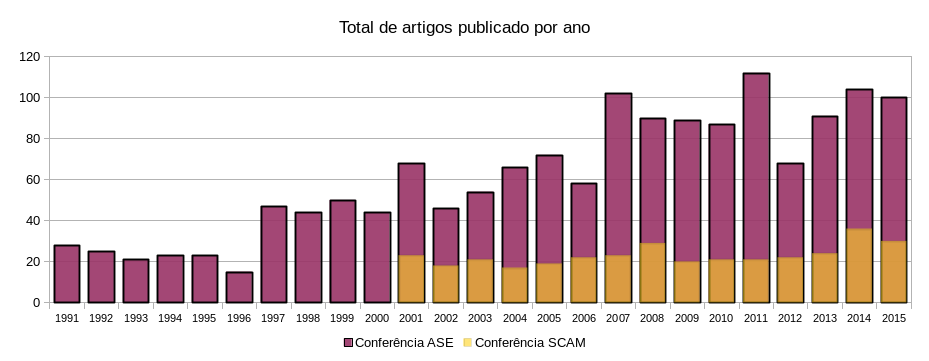
\includegraphics[scale=0.65]{imagens/artigos-por-ano.png}
  \caption{Total de artigos por ano publicados nas conferências ASE e SCAM.}
  \label{artigos-por-ano}
\end{figure}

  \item [Passo 2: Triagem Automática]

Até o ano de 1996, nenhum artigo foi encontrado na conferência ASE com
ocorrência das palavras-chave utilizadas no filtro. Apenas a partir de 1997
temos ocorrência dos termos pesquisados nas publicações desta conferência.

  \item [Passo 3: Extração]

Considerando todo o período incluído na revisão de literatura, encontramos uma
média de 2 artigos por ano com publicação de software acadêmico. A Figura
\ref{artigos-com-software-por-ano} apresenta os resultados distribuídos por
ano.

\begin{figure}[h]
  \center
  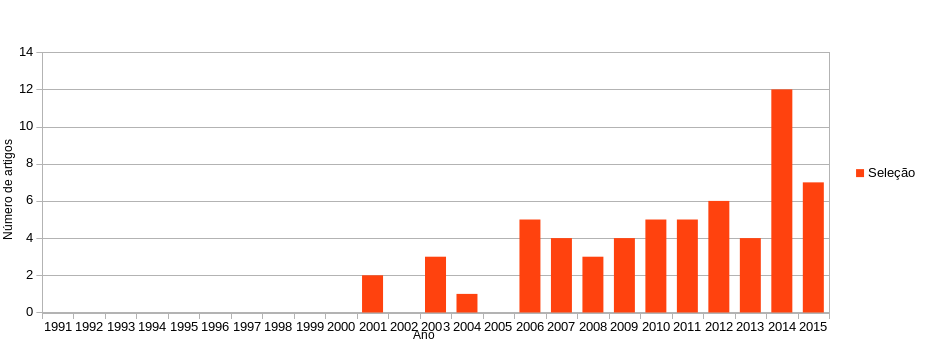
\includegraphics[scale=0.65]{imagens/artigos-com-software-por-ano.png}
  \caption{Artigos com publicação de software acadêmico selecionados na revisão de literatura.}
  \label{artigos-com-software-por-ano}
\end{figure}

A revisão de literatura teve como critério primordial encontrar publicação de
software com indicação de URL para download; ainda assim, no processo de
revisão, encontramos 51 projetos sem indicação de URL para download, sendo 30 projetos
na conferência ASE e 21 projetos na conferência SCAM.

\end{description}

% }}}

\section{Interpretação dos Resultados} \label{estudo1:interpretacao} % {{{

\subsection{Q1 - \EstudoUmQuestaoUm} % presença online

Dos \SoftwareCount \ projetos de software estudados neste trabalho, \SoftwareUrlNotAvailableCount \ não têm presença
oficial online no endereço de URL informado pelos seus autores, \SoftwareUrlAvailableCount \ projetos
estão presentes através da URL informada de alguma forma, significando que as
URL informada pelos autores estão ativas e online.

\subsection{Q2 - \EstudoUmQuestaoDois} % download

Entre os \SoftwareCount \ projetos selecionados, 24 não estão disponíveis para download, ou
seja, apesar dos autores informarem no estudo uma URL, indicarem que o software
está disponível nesta URL para download, a URL não mais está disponível e o
software não pode ser encontrado. Isso significa que 40\% dos projetos de software
acadêmico de análise estática publicados nas conferências de Engenharia de
Software ASE e SCAM não estão disponíveis.

Os demais 36 projetos, que equivalem a 60\% do conjunto total, estão
disponíveis para download e é possível obter uma cópia destes projetos na URL
indicada pelos seus autores. Um resumo deste total por ano é apresentado na
Tabela \ref{available-table}.



\begin{table}[h]
\caption{Número de projetos disponível para download por ano.}
\centering
\begin{tabular}{l c c c}
  \hline
  {\bf Ano} & {\bf Total} & {\bf Disponível} & {\bf Indisponível} \\
  \hline
  2001 & 2 & 1 & 1 \\
  2003 & 3 & 1 & 2 \\
  2004 & 1 & 0 & 1 \\
  2006 & 5 & 4 & 1 \\
  2007 & 4 & 1 & 3 \\
  2008 & 2 & 1 & 1 \\
  2009 & 4 & 2 & 2 \\
  2010 & 5 & 3 & 2 \\
  2011 & 5 & 2 & 3 \\
  2012 & 6 & 2 & 4 \\
  2013 & 4 & 2 & 2 \\
  2014 & 12 & 11 & 1 \\
  2015 & 7 & 6 & 1 \\
  \hline
  {\bf Total} & 60 & 36 & 24 \\
  \hline
\end{tabular}
\label{available-table}
\end{table}



\subsection{Q3 - \EstudoUmQuestaoTres} % codigo fonte

Do conjunto de 36 projetos de software disponíveis para download, apenas 2 não
disponibilizam o código fonte. Tais projetos -- FaultBuster e Loopfrog --
são disponibilizados gratuitamente mas apenas em
formato binário. A Tabela \ref{source-code-table} traz um resumo das
linguagens de programação usadas para a implementação dos projetos de software.

\begin{table}[h]
\caption{Linguagem de programação dos projetos com código-fonte disponível.}
\centering
\begin{tabular}{l c}
  \hline
  {\bf Linguagem de programação} & {\bf Número de projetos} \\
  \hline
  C & 6 \\
  C++ & 2 \\
  Erlang & 1 \\
  Java & 18 \\
  Javascript & 2 \\
  Perl & 1 \\
  Python & 2 \\
  Rascal & 1 \\
  Ruby & 1 \\
  \hline
  {\bf Total} & 34 \\
  \hline
\end{tabular}
\label{source-code-table}
\end{table}


\subsection{Q4 - \EstudoUmQuestaoQuatro} % licença

Dentre os 34 projetos que disponibilizaram o código fonte, 13 não informaram
licença alguma e 21 informaram licenças de FOSS ({\it free and open source
software}). A Tabela \ref{license-table} resume as licenças utilizadas e o
número de projetos em cada uma.

\begin{table}[h]
\caption{Licenças de software dos projetos com código fonte disponível.}
\centering
\begin{tabular}{l c}
  \hline
  {\bf Licença de software} & {\bf Número de projetos} \\
  \hline
  Affero General Public License & 1 \\
  Apache License & 2 \\
  BSD License & 4 \\
  Eclipse Public License & 3 \\
  FrontEndART Software Ltd & 1 \\
  GNU General Public License & 6 \\
  GNU Lesser General Public License & 1 \\
  Illinois/NCSA Open Source License & 2 \\
  SAnToS Laboratory Open Academic License & 1 \\
  (sem licença) & 13 \\
  \hline
  {\bf Total} & 34 \\
  \hline
\end{tabular}
\label{license-table}
\end{table}


Todo software com o código fonte disponível pode ser adaptado para uso pessoal
sem qualquer restrição prévia pelos seus autores, mas os 13 projetos sem
licença definida impedem eventuais cientistas a publicar suas modificações e
redistribuir qualquer melhoria sem prévia solicitação aos autores originais.

Considerando o total de 60 projetos selecionados neste estudo, apenas 35\% (21
projetos) podem ser adaptados; os demais com código fonte disponível, 21\% (13 projetos) podem ser
adaptados, mas as melhorias ou correções não podem ser redistribuídas sem
autorização prévia dos autores.

% }}}

\section{Ameaças à Validade} % {{{

O passo de triagem automática dos artigos no processo de revisão de literatura
pode ter excluído do processo de revisão algumas publicações com software
acadêmico de análise estática, 
não incluindo algum software acadêmico publicado no conjunto total de projetos
selecionados. Apesar disso, o estudo tem como objetivo
caracterizar os projetos e não as conferências em sí, de forma que esta ameaça
não causa impacto nas conclusões finais do estudo.

O escopo do estudo foi reduzido ao domínio de análise estática, portanto as
conclusões e interpretações estão limitadas neste contexto. Acreditamos que
outros domínios de aplicação possuem características semelhantes, mas é
conhecido que o domínio de aplicação pode ser um fator de influência relevante nas
características dos produtos de software.
Por exemplo, \citeonline{zhang2013how}, num estudo sobre como o contexto afeta
a distribuição de métricas de manutenibilidade, conclui que os maiores fatores
de influencia são o domínio de aplicação, a linguagem de programação e o número
de mudanças.

A leitura dos artigos na fase final de Extração, foi realizada
apenas pelo autor deste trabalho. Tal ameaça poderia ter sido minimizada com
revisão em par, ou por outros pesquisadores.

O contexto selecionado com apenas duas conferências nos leva a possibilidade de
ter resultados com viés atrelado a estes dois eventos; é possível que as
características dos projetos publicados em outras conferências da Engenharia de
Software apresentem situação diferentes.

A avaliação da disponibilidade do software para download usando apenas a URL
informada pelos seus autores pode levar a falso-negativos, uma vez que é
possível a URL mudar com o tempo, esta ameaça apesar de não ter sido
tratada não invalida nossas conclusões, uma vez que o estudo teve como objetivo
inicial avaliar primariamente a própria URL indicada pelos autores originais.

% }}}

\section{Conclusões} \label{estudo1:conclusoes} % {{{

Este estudo selecionou 60 projetos de software de análise estática de código
fonte publicados nas conferências ASE e SCAM, todos identificados com nome do
projeto e URL para download. Os autores afirmam que os projetos estão
disponíveis para obtenção na URL indicada, mas os resultados da caracterização
feita mostram que apenas uma parcela destes projetos continuam disponíveis.

Entre os 60 projetos selecionados, 15 não têm qualquer presença oficial online,
com a URL indicada pelos autores indisponível. As únicas informações
disponíveis destes 15 projetos são aquelas encontradas nos artigos onde foram
publicados.

Nos 45 projetos com presença online através da URL informada nos artigos, 9 não
disponibilizam qualquer artefato relacionado ao software, ou seja, apesar de
ser possível acessar a URL, não é possível encontrar o software para download.
Os outros 36 projetos estão disponíveis para download, sendo que
a maior parte, 34 projetos, disponibiliza o código fonte, e apenas 2
estão disponíveis em formato binário.

Dentre os 34 projetos com código fonte disponível, 13 não informam qualquer
licença de uso e, dessa forma, impedem que melhorias e correções
sejam distribuídas sem antes haver uma solicitação prévia aos autores destes
projetos. Finalmente, 19 projetos utilizam licenças de software livre e dão
prévia autorização para receber melhorias em código fonte.

É conhecido que os projetos de software desenvolvidos na academia não são ainda
reconhecidos pela Ciência como cidadãos de primeira classe, mesmo quando tais
projetos são indispensáveis para a compreensão dos estudos em que foram
desenvolvidos. Neste estudo mostramos que uma grande parte (40\%) de um
conjunto de projetos de software acadêmico minimamente identificados pelos seus
autores com nome e URL encontra-se hoje indisponível.

No entanto, não sabemos quais os fatores que influenciam um projeto estar ou não
disponível, e ainda, como tais projetos são vistos por outros pesquisadores, ou se
são utilizados e referenciados por outros autores. Assim planejamos outros
estudos para investigar tais questões, apresentados nos próximos capítulos.

% }}}
